%%%%%%%%%%%%%%%


Through its effect on drift velocity, recombination, and lifetime, the \efield is a critical parameter for physics signals as it ultimately affects the spatial resolution and energy response of the detector. The primary purpose of a laser system is to provide an independent, fine-grained estimate of the \efield in space and time. It would be extremely valuable to achieve measurements of electron lifetime with the laser system, but the feasibility of that is still under discussion.
The R\&D plan in \dword{pddp} will address the feasibility of carrying out charge-based measurements which, if successful, would open up the possibility of using the laser to measure electron lifetime. So, except where specifically indicated, the rest of this section will focus on drift velocity and \efield measurement.

\subsubsection{Physics Motivation}
Because it measures spatial distortions of straight tracks, the laser system actually measures the local drift velocity field directly and helps define the detector \dword{fv}, and this in itself is an important input for the \dword{lbl} analysis. 
%, and this is in itself an input to the analysis.
%Still,
However, it is still important to use information independent of the charge in order to disentangle effects like lifetime and recombination from \efield distortions. The laser system can do this, by using the position information to derive the \efield from the local velocity map, taking into account the colinearity between both vectors, and the relatively well studied relation on the magnitude (see~\cite{Li:2015rqa} and references [29, 45-58] therein). A laser system also has the intrinsic advantage of being immune to recombination, thus eliminating particle-dependent effects.  


Several sources may distort the drift \efield temporally and/or spatially in the detector. Positive ion accumulation and drift (space charge) due to ionization sources like cosmic rays or \Ar39 should be significant in the \dword{dune} \dword{dp} \dword{fd} module. Current simulation studies indicate that, considering only the accumulation of positive ions created in the liquid phase, we should expect \efield distortions of at most \SI{1}{\%}~\cite{bib:mooney2018}. Because of the longer drift length this is already significantly more than the \SI{0.1}{\%} expected in \dword{sp}. In addition, a fraction of the positive ions created in the gas phase amplification stage can drift back into the liquid and cause even more distortion. Current studies\footnote{These studies are based on the following assumptions: \dword{lem} gain of \num{100}; \SI{10}{\%} of the ions from gas phase drift into \lar; ion drift velocity of \SI{8}{\milli\metre\per\s}.} indicate that the \efield distortion caused by space charge, including ion feedback, can reach \SI{15}{\%} of the nominal field~\cite{bib:yu2018a}.
Furthermore, this effect may be enhanced or spatially distorted because of possible stable eddies in the \dword{lar} fluid flow. A \SI{15}{\%} distortion can lead to spatial distortions of \SI{1.2}{\metre} and temporal distortions of \SI{0.1}{\milli\s}, which are very significant compared to \dword{sp}. 
%KMTDRREADME: most 1% => at most 1%

%However, not enough is known yet about the fluid flow pattern in the \dword{fd} to exclude the possibility of stable eddies which may amplify the effect for both \single and \dual modules. This effect can get further amplified significantly in the \dword{dpmod} due to  accumulation in the liquid of ions created by the electron multiplication process in the gas phase.
%due to ion accumulation at the liquid-gas interface. 
Additionally, other sources in the detector (especially detector imperfections) can cause \efield distortions. For example, \dword{fc} resistor failures (see Figure~\ref{fig:efield_resistorfailure_mooney2019}), non-uniform resistivity in the voltage dividers, and misalignment or structural deformations of the cathode grid can create localized \efield distortions. These effects should be less pronounced than in the \dword{sp} because there are fewer detector elements within the \dword{tpc}, but also because in the \dword{dp} system, four resistors would have to fail to cause a failure across the \dword{fc} gap.

%\begin{dunefigure}[Impact on \efield of \dword{cpa} position distortions]{fig:efield_cpa_distortions_boyu2017}
%{Illustration of a possible distortion of the \dword{cpa} position~\cite{bib:yu2017a}, assuming a \SI{2}{\cm} swing, and its impact on \efield (right).}
%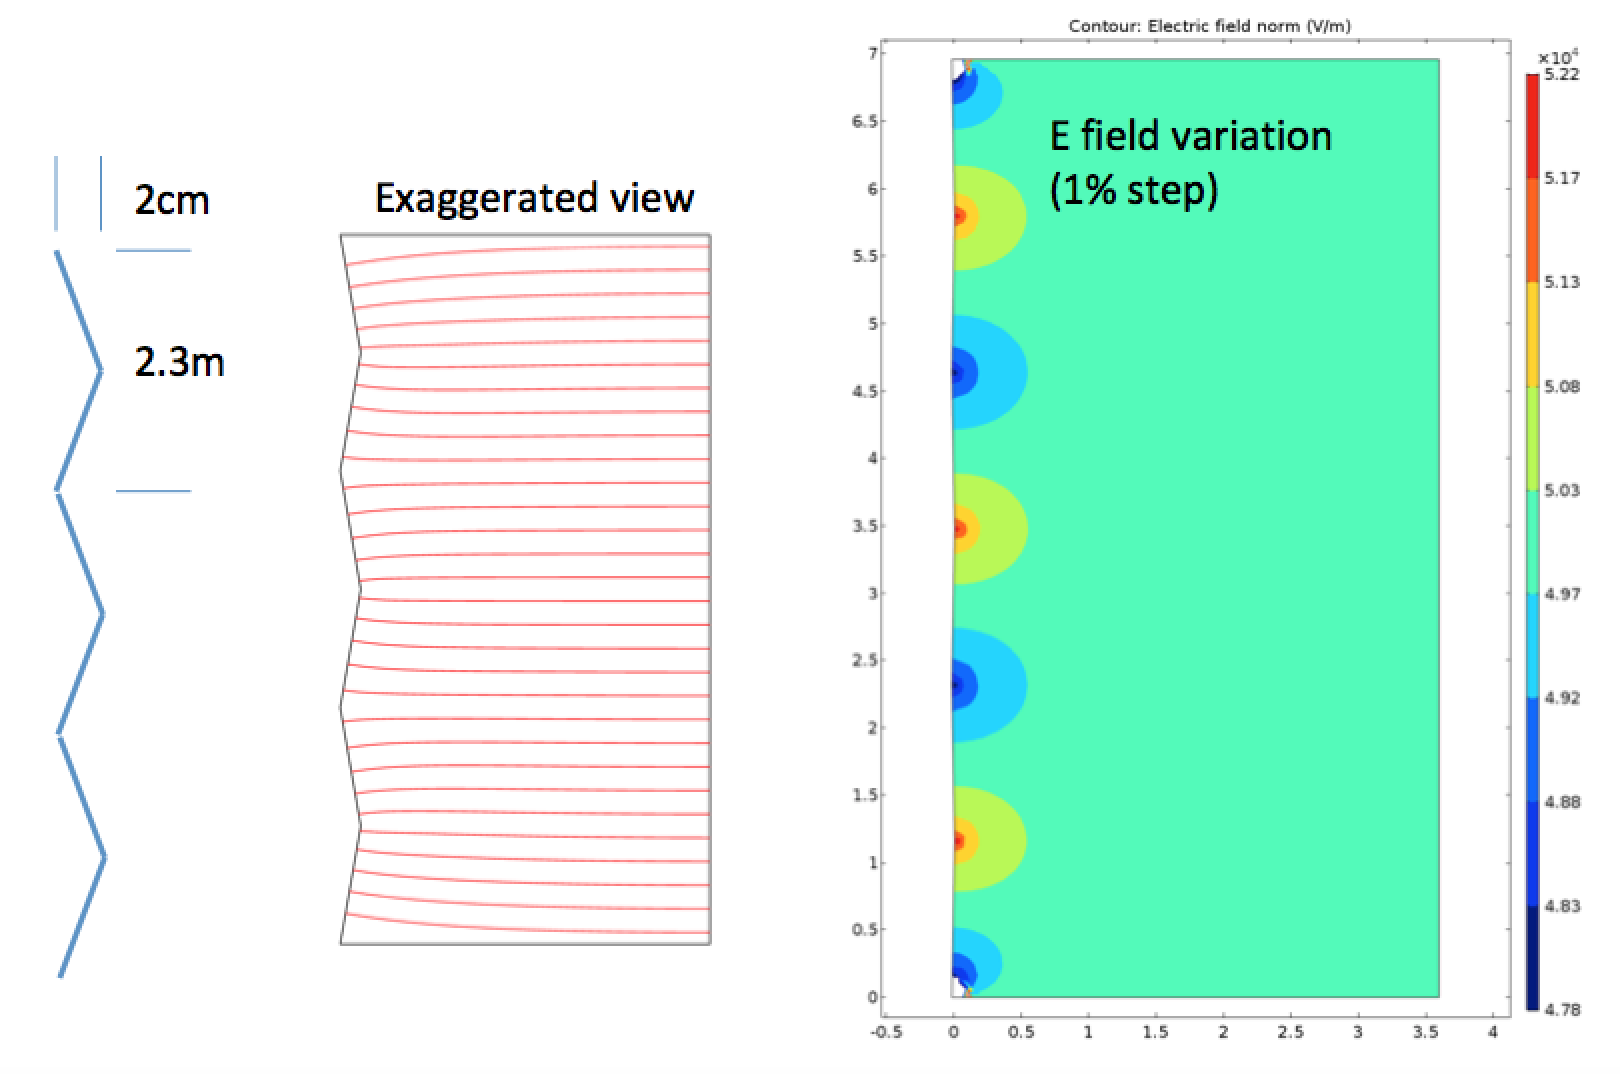
\includegraphics[width=0.8\textwidth]{efield_cpa_distortions_boyu2017.png}
%\end{dunefigure}

\begin{dunefigure}[Effect on \efield of  \dshort{fc} resistor failures]{fig:efield_resistorfailure_mooney2019}
{Effect on \efield magnitude distortions of a single \dword{fc} resistor failure in \dword{pdsp}~\cite{bib:mooney2019a}; shown as an example. 
%Caveat: Calculation done for \dword{sp}.
}
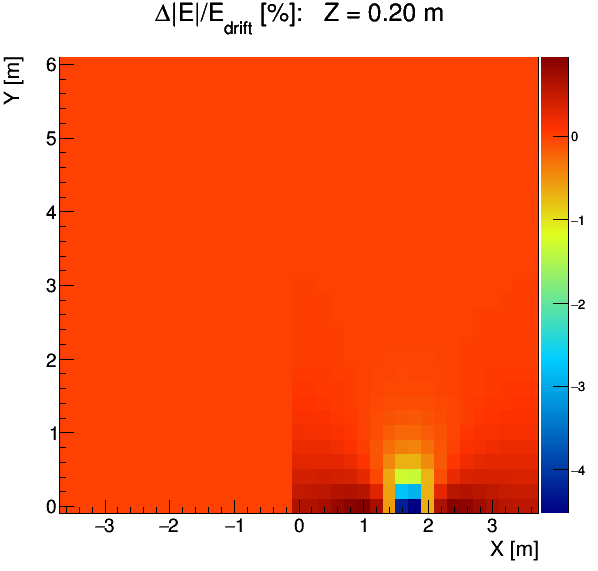
\includegraphics[width=0.5\textwidth]{efield_resistorfailure_mooney2019.png}
\end{dunefigure}

%In both \single and \dual systems, the failure of a resistor will create significant, local electric field distortions which will need to be identified\footnote{In the \dual system, four resistors would have to fail to cause a failure across the field cage gap, but even one failure in the SP can have an impact; this may be partially mitigated by modifying the HV, but not completely.}. While the resistor failure will be detected temporally, its location in space is not possible to determine from slow controls monitoring data. Misalignments of detector objects or deformations may also create (small) electric field distortions; while individual effects may be small, it is possible to have a combined, significant effect.

%KMTDRREADME, removed the 15% which seemed redundant with above.
Even if ion feedback space charge is expected to be the dominant \efield distortion effect,
%by up to \SI{15}{\%},
each individual \efield distortion may contribute, causing localized effects that must be understood with \textit{in situ} measurements of \efield for proper calibration. 

The laser system has many useful secondary uses as well, including alignment (especially for modes weakly constrained by cosmic rays),
%; see Figure~\ref{fig:apacurtainalign}),
stability monitoring, and diagnosing detector performance issues
%failures 
(e.g., \dword{hv}).  
%Misalignment may include physical deformation and/or rotations of objects within the detector.
Given the expected low rate of cosmic ray events (about 3500/day/10-kt) at the underground location, calibration with cosmic rays is not possible over short time scales. 
%KMTDRREADME: Add duration of timescale? Maybe "A 1% measurement is possible on a year timescale" Do we want to comment on rotation elements? Are there any?

%A laser system also has the intrinsic advantage of being immune to recombination, thus eliminating particle-dependent effects.  

With respect to electron lifetime, the preliminary results from \dword{pdsp} purity monitors and cosmic ray analyses indicate significant variations with time and space, both between monitors at different vertical coordinates (see \dword{tdr} \spchcisc), and between the regions inside and outside the \dword{tpc}. The possibility of carrying out such measurements with the ionization laser is therefore quite interesting. The ArgonTUBE experiment obtained lifetime measurements with laser~\cite{Ereditato:2013xaa} compatible with the cosmic ray ones, but it is not clear yet if this is possible at very large scales, since the modelling of the density of ionization charge created along the tracks presents challenges related to the previously mentioned self-focusing. Therefore the characterization of the ionization charge density from laser tracks will be an important goal of the development plan in \dword{pddp}.



%%%%%%%%%%%%%%%%%%%%%%%%%%%%
\subsubsection{Requirements}
\label{sec:dp-calib-laser-req}

%\fixme{uncomment when spec table available.\\ JM: but the spec table is included in a previous section, within overview.tex. I think the name requirements.tex is misleading. I'm changing to laser-ionization-requirements.tex; SG: agreed.}

% KM outline
%% Requirements we are held to from other systems -- EB table -- see Jose's early talk
%% Targets for SN and LBL physics -- or just remind in other subsections? \fixme{KM: right now the targets for SN and LBL physics exist in the design sections.}
%% System must operate for a long time
    % SG: physics driven calibration requirements, need a table to connect calibration requirements to high level physics requirements, not easy, but we need to try

%\fixme{guidance coming soon!}

%\fixme{KM: adjusted to be specific to laser; SG: I have made some edits as well. JM: OK, signing off.}

%The DUNE physics requirements and the high level specifications of other existing systems are the driving motivation for the specifications of the performance of the dedicated calibration systems, described below. From those, and the constraints due to detector dimensions, etc, derive also the engineering specifications of each calibration system, described in each system's respective section.

%\paragraph{\efield measurements}
The energy and position reconstruction requirements for physics measurements lead to requirements on the necessary precision of the laser %calibration 
\efield measurement, its spatial coverage and granularity. The next sections discuss the rationale behind each requirement, which we take as the \dword{dune} specification.
%, with ALARA (or AHARA for the coverage) as goal.

\paragraph{\efield precision}

In the \dword{lbl} and high-energy range, \physchlbl of this \dword{tdr}
%the \dword{dune} physics \dword{tdr} 
states that the calibration information must provide approximately \num{1} to \SI{2}{\%} understanding of normalization, energy scale and resolution, and position resolution within the detector.
Because a smaller \efield leads to higher electron-ion recombination and therefore a lower collected charge, distortions of the \efield can introduce
%are one of the possible causes of an 
energy scale bias. To connect this
%that requirement 
to a specification for the necessary precision of the \efield measurement, we note that, via recombination studies~\cite{bib:mooney2018}, we expect a \SI{1}{\%} distortion on \efield to lead to a \SI{0.3}{\%} bias on collected charge.
Because other effects will contribute to the lepton energy scale uncertainty budget, we consider a goal for the 
%calibration 
laser system to measure the \efield to a precision of $\sim$\SI{1}{\%} so that its effect on the collected charge is well below \SI{1}{\%}.
This is also motivated by the need for consistency with the high level \dword{dune} specification for field uniformity throughout the volume due to component alignment and \dword{hv} system, set at \fielduniformity. As was mentioned in Section~\ref{sec:dp-calib-requirements}, in \dword{dp} the long drift length and the gas phase ion feedback will lead to larger space charge \efield distortions than in \dword{sp}, up to approximately \SI{15}{\%}, making it even more important in \dword{dp} to monitor the \efield although the precision requirement should be the same (\SI{1}{\%}), as determined by the physics requirements, not by instrumentation constraints.

With two other high-level \dword{dune} specifications, the \dword{crp} strip spacing (\dpstrippitch) and the front end peaking time (\fepeaktime), the effect of this \efield precision requirement on engineering parameters of the calibration laser system is discussed further %ahead, 
in Section~\ref{sec:dp-calib-sys-las-ion-meas}.

\paragraph{\efield measurement coverage:}

In practice, measuring the \efield  throughout the whole volume of the \dword{tpc} will be difficult, so we must establish a goal for the coverage and granularity of the measurement. 
Until a detailed study of the propagation of the coverage and granularity into a resolution metric is available, a rough estimate of the necessary coverage can be made as follows.

Assuming \SI{15}{\%} as the maximum \efield distortion from possible compounding multiple  effects in the \dword{dune} \dword{fd},
we can then ask what would be the maximum acceptable size of the spatial region uncovered by the calibration system, if a distortion of that magnitude (systematically biased in the same direction) were present. To keep the overall (average) \efield distortion at the \SI{1}{\%} level, then that region should be no larger than \SI{7}{\%} of the total \dword{fv}. Therefore, we need a coverage of \SI{93}{\%} or more.

In addition, we need to consider that the method used to estimate \efield distortions is based on obtaining position displacement maps~\cite{bib:uBlaser2019}, and that the comparison between the reconstructed and true direction of a single track does not %univocally %unequivocally 
unambiguously determine a specific displacement map. Having tracks coming from different origins crossing in the same position is a direct way to eliminate that ambiguity, since the displacement vector is given simply by the vector connecting the intersections of the two reconstructed and the two true tracks. A joint iterative analysis of several close-by tracks is the default method for all other positions, but the system design should allow for the maximum possible number of positions %where there can be 
for crossing tracks from different beams.


\paragraph{\efield measurement granularity:}

The Volume~\volnumberphysics~(\voltitlephysics) of this \dword{tdr} states that a \dword{fv} uncertainty of \SI{1}{\%} is required. 
This translates to a position uncertainty of \SI{1.5}{\cm} in each coordinate (see \dword{tdr} \spchapa). 
In the $y$ and $z$ coordinates, position uncertainty is given mainly by the \dword{crp} strip pitch, and since this is \dpstrippitch, the requirement is met even when added in quadrature to the estimated maximum lateral diffusion of \SI{4.4}{\milli\m}. In the drift ($x$) direction, the position is calculated from timing, and considering the electronics peaking time of \fepeaktime, the uncertainty should be even smaller.
%\fixme{This is not entirely clear, and I can't see how to rephrase it.}
%\fixme{JM: Re-tweaked, I think it's clearer now. Please remove both if OK.}

The position uncertainty, however, also depends on the \efield, via the drift velocity. Because the position distortions accumulate over the drift path of the electron, it is not enough to specify an uncertainty on the field. We must accompany it by specifying the size of the spatial region of that distortion. For example, a \SI{10}{\%} distortion would not be relevant if it was confined to a \SI{2}{\cm} region and if the rest of the drift region was at nominal field.

Therefore, what matters is the product of [size of region] $\times$ [distortion]. Moreover, one can distinguish distortions into two types:
\begin{enumerate}
\item Those affecting the magnitude of the field. Then the effect on the drift velocity $v$ is also a change of magnitude. According to the function provided in \cite{Walkowiak:2000wf}, close to \SI{500}{\V\per\cm}, the variation of the velocity with the field is such that a \SI{4}{\%} variation in field $E$ leads to a \SI{1.5}{\%} variation in $v$.
\item Those affecting the direction of the field. Nominally, the field $E$ should be along $x$, so $E = E_L$ (the longitudinal component). If we consider that the distortions introduce a new transverse component $E_T$, in this case, this translates directly into the same effect in the drift velocity, which gains a $v_T$ component, $v_T=v_L  E_T/E_L $, i.e., a \SI{4}{\%} transverse distortion on the field leads to a \SI{4}{\%} transverse distortion on the drift velocity.
\end{enumerate}

Thus, a \SI{1.5}{\cm} shift comes about from a constant \SI{1.5}{\%} distortion in the velocity field over a region of \SI{1}{\m}. For the \efield, that could be from a \SI{1.5}{\%} distortion in $E_T$ over \SI{1}{\m} or a \SI{4}{\%} distortion in $E_L$ over the same distance.

%From ref.~\cite{Abi:2018dnh}, page~4-53, 
\efield distortions can be caused by space-charge effects due to accumulation of positive ions caused by \Ar39 decays (cosmic ray rate is low in \dword{fd}), or detector defects, such as \dword{crp} or \dword{fc} misalignment, \dword{fc} resistor failures (Figure~\ref{fig:efield_resistorfailure_mooney2019}), and resistivity non-uniformities, among other things.
%~\cite{Abi:2018dnh}. 
These effects added in quadrature can be as high as \SI{4}{\%}. 
%From ref. ~\cite{bib:mooney2018}, 
The space charge effects due to \Ar39~\cite{bib:mooney2018} can be \SI{0.1}{\%} for the \dword{sp} and \SI{1}{\%} for the \dword{dp}, so in practice, these levels of 
%that kind of distortion 
distortions must cover several meters to be relevant.
Other effects due to \dword{fc} imperfections can be higher than those due to space charge, but they are also much more localized. If we assume no foreseeable effects would distort the field more than \SI{15}{\%}, and considering the worst case scenario (transverse distortions), then the smallest region that would produce a \SI{1.5}{\cm} shift is \SI{1.5}{\cm}/\num{0.15}~=~\SI{10}{\cm}. This provides a target for the granularity of the measurement of the \efield distortions in $y$ to be smaller than about \SI{10}{\cm}, with of course a larger region if the distortions are smaller. Given the above considerations, then a voxel size of \num{10}$\times$\num{10}$\times$\SI{10}{\cubic\cm} appears to be enough to measure the \efield with the granularity needed for a good position reconstruction precision. 
%In fact, since the effects that can likely cause bigger \efield distortions are the problems or alignments in the \dword{cpa} (or \dword{apa}), or in the \dword{fc}, it could be conceivable to have different size voxels for different regions, saving the highest granularity of the probing for the walls/edges of the drift volume.



\begin{comment}
\begin{dunetable}
[Calibration Requirements]
{p{0.5\textwidth}p{0.15\textwidth}p{0.15\textwidth}}
{tab:calibreq}
{Calibration Specifications and Goals}   
Requirement & Specification & Goal \\ \toprowrule
\efield measurement precision & < 1\% & ALARA \\ \colhline
\efield measurement coverage & > 93\% & AHARA \\ \colhline
\efield measurement granularity & < 10x10x10 cm & ALARA \\ \colhline
\end{dunetable}
\end{comment}



\subsubsection{Design}
\label{sec:sp-calib-sys-las-ion-des}
%\paragraph{Baseline design}

The design of the laser calibration system for \dword{dune} is largely based on the design of the system built for \dword{microboone}~\cite{microboone}, which in turn was based on several previous developments~\cite{Rossi:2009im,Zeller:2013sva,Ereditato:2014lra,Ereditato:82014tya}. A similar system was also built for \dword{captain}~\cite{Berns:2013usa} and in the near future, will be built for \dword{sbnd}~\cite{Antonello:2015lea}. Operation of the \dword{microboone} system has already taken place. A preliminary report was given in~\cite{bib:chen2018}, and more details on the data analysis are available in~\cite{bib:uBlaser2019}.
%\todo{link the reference once uB publishes the laser paper in 2019}

\paragraph{Design overview}
Ionization of \dword{lar} by laser can occur via a multiphoton process in which two-photon absorption~\cite{Badhrees:2010zz} leads the atom to the excited states band, and a third photon subsequently causes ionization. This can only occur with high photon fluxes, and so the lasers must provide pulse energies of \SI{60}{\milli\joule} or more within a few ns. Unlike muons, the laser beams do not suffer multiple scattering and travel along straight lines determined by the steering mirror optics. 
The basic measurement consists of %recording the laser beams 
generating laser ionization tracks in the \dword{tpc} and comparing the reconstructed tracks with the direction known from the steering hardware. 
An apparent curvature of the measured track is attributed to drift velocity, and therefore \efield, distortions (either in direction or magnitude).


%Send this to last section
%The first step in the analysis~\cite{bib:uBlaser2019} is to obtain a field of position displacements by comparing the known and reconstructed tracks. If two crossing tracks are used, the displacement vector is simply given by the vector connecting the point where the reconstructed tracks cross and the point where the known tracks cross. However, because those displacements can vary both in direction and magnitude, that determination is ambiguous if only one track is used in a given spatial region. An iterative procedure was developed by the \dword{microboone} collaboration~\cite{bib:chen2018,bib:uBlaser2019} to 
%still 
%obtain a displacement map from a set of several non-crossing tracks from opposite directions. Following this, a set of drift velocity field lines (also known as \efield lines) can be obtained from the displacement map, assuming that all charge deposits along a field line will be collected in the same position. Using the relationship between \efield and drift velocity~\cite{Li:2015rqa,Walkowiak:2000wf}, the magnitude of the \efield can then be obtained 
%as well 

While the Rayleigh scattering length for \SI{266}{\nano\m}  light is approximately \SI{40}{\m}, additional optics effects may limit the maximum practical range of laser beams of that wavelength to a distance smaller than that. Those can include the Kerr effect  due to the dependency of the refractive index on the \efield. In the presence of an intense field, such as that caused by the laser beam itself, the change in refractive index can lead to lensing, or focusing, that distorts the coherence of the beam\footnote{The Kerr effect is so far believed to be the cause of non-homogeneity of the ionization along the laser beam observed in \dword{microboone}, which prevents the use of the charge information. Its effect on the position measurement and \efield uncertainty has been studied by \dword{microboone}.}. 

Despite this, laser beams with lengths of \SI{10}{\m} in \dword{lar} have been observed in \dword{microboone}, and beams with \SI{20}{\m} lengths (possibly more) can be reasonably expected to obtain with a similar system. This has determined the choice of locating the calibration ports in the cryostat roof at \SI{12}{\m} intervals. The \dword{dune} \dword{dp} cryostat roof port map is not defined yet, but the calibration proposal will have two sets of \num{6} ports located above the north and south walls, for a total of \num{12} ports, as shown in Figure~\ref{fig:DPFDLaserPositions}.

\paragraph{Mechanical and optical design for a single port sub-system}

For each of %those 
the used calibration ports, a laser sub-system can be schematically represented by Figure~\ref{fig:uB_laser_schematic} (left) and consists of the following elements:
\begin{itemize}
    \item a laser box (see Figure \ref{fig:uB_laser_schematic}, right) that provides
    \begin{itemize}
        \item a Nd:YAG laser, with the fourth harmonic option providing \SI{266}{\nano\m} in intense \SI{60}{\milli\joule} pulses with about \SI{5}{\nano\s} width, with a divergence of \SI{0.5}{\milli\radian}. The Surelite SL I-10 laser\footnote{Amplitude Surelite\texttrademark{} https://amplitude-laser.com/wp-content/uploads/2019/01/Surelite-I-II-III.pdf} is a possible choice since it has been successfully used in the past in other experiments.
        \item an attenuator and a collimator to control the intensity and size of the beam;
        \item a photodiode that gives a \dword{tpc}-independent trigger signal;
        \item a low-power red laser, aligned with the UV laser, to facilitate alignment operations; and
        \item a Faraday cage to shield the surrounding electronics from the accompanying electromagnetic pulse. %EM \fixme{EM is defined as emergency management in the common glossary. Perhaps this should be spelled out? (Anne agrees and fixed.}
    \end{itemize}
    \item a feedthrough (see Figure \ref{fig:uB_laser_ft}, left) into the cryostat that provides
    \begin{itemize}
        \item the optical coupling that allows the UV light to pass through into the cryostat directly into the liquid phase, avoiding distortions due to the gas-liquid interface and the gas itself;
        \item a rotational coupling that allows the whole structure to rotate while maintaining the cryostat seal;
        \item a periscope structure (see Figure~\ref{fig:uB_laser_ft}; Right) mounted under the rotating coupling that supports a mirror within the \dword{lar};
        \item the additional theta rotation of the mirror accomplished by a precision mechanism coupled to an external linear actuator; and
        \item both the rotation and linear movements of the steering mechanism read out by precision encoders.
    \end{itemize}
    
\end{itemize}

\begin{dunefigure}[\dshort{microboone} laser calibration system schematics]{fig:uB_laser_schematic}
{Left: Schematics of the ionization laser system in one port~\cite{Antonello:2015lea}. Right: Schematics of the laser box~\cite{microboone}.}
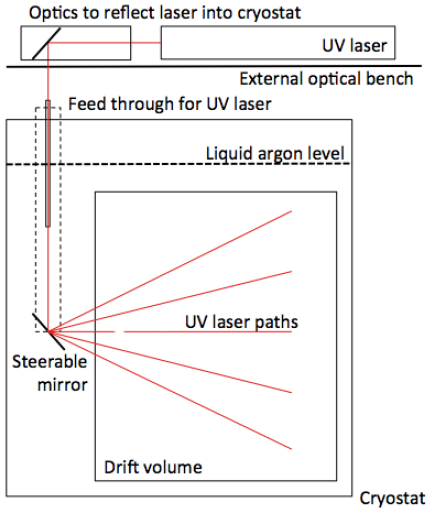
\includegraphics[width=0.45\linewidth]{uB_laser_schematic}
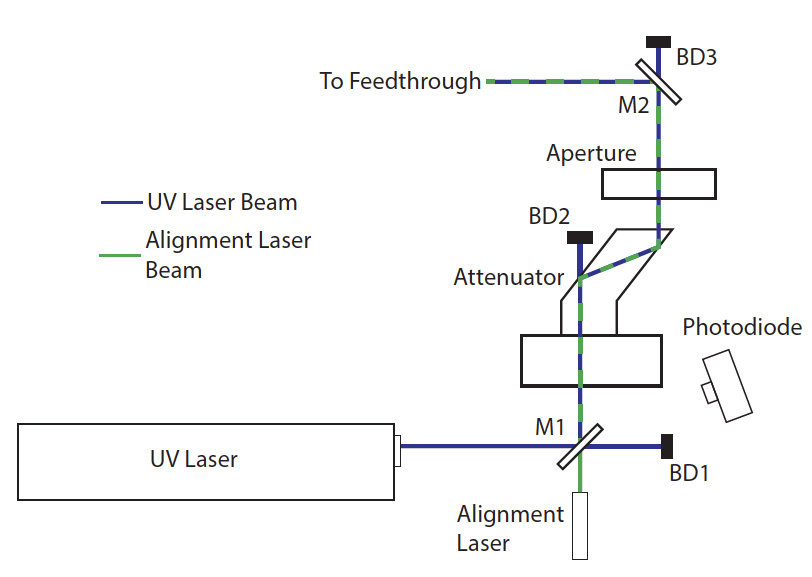
\includegraphics[width=0.5\linewidth]{uB_laser_box}
\end{dunefigure}

\begin{dunefigure}[\dshort{microboone} laser calibration system drawings]{fig:uB_laser_ft}
{CAD drawings of the \dword{microboone} laser calibration system~\cite{microboone}. Left: calibration port feedthrough. Right: laser beam periscope. %Both figures from~\cite{microboone}.
}
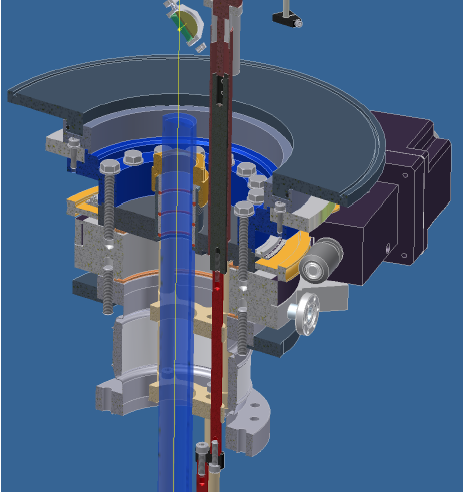
\includegraphics[width=0.49\linewidth]{uB_laser_ft}
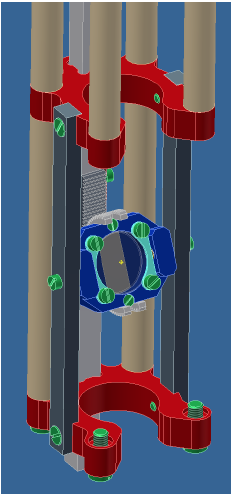
\includegraphics[width=0.248\linewidth]{uB_laser_periscope}
\end{dunefigure}

The baseline design will have the periscopes entering the top of the \dword{tpc} through the gap %space 
between the \dword{fc} and the \dword{crp} (see the views in figures \ref{fig:LaserPositionCorner} and \ref{fig:LaserPositionSide}). The brackets that connect the \dword{fc} structural elements (light grey and blue in the figures) must be adapted with suitable size holes that allow for the periscope size and a tolerance for the shifts due to \dword{fc} thermal shrinkage. This design allows \num{12} periscopes inside the \dword{tpc}, with no shadowing elements blocking the laser beams from covering the full volume.

\begin{dunefigure}[Laser calibration periscopes in the  \dshort{dp} \dshort{tpc} corner]{fig:LaserPositionCorner}
{CAD illustration of the calibration periscopes within the \dword{dune} \dword{dp} \dword{tpc} corner. Left: View from top. Right: View from bottom.}
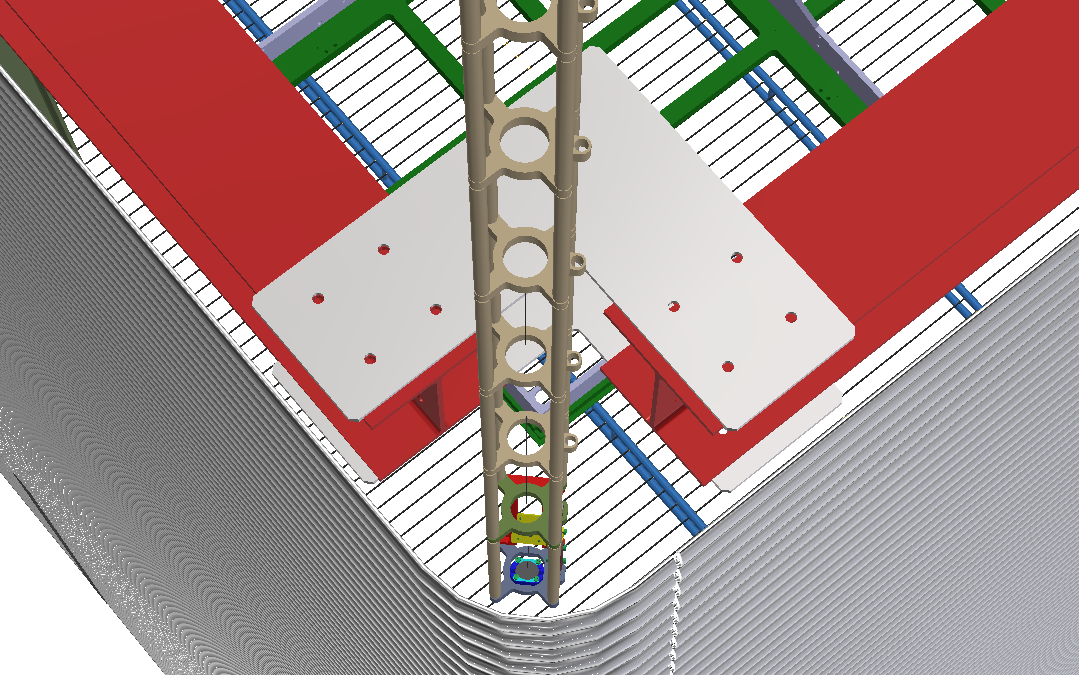
\includegraphics[width=0.49\linewidth]{LaserPositionCorner.png}
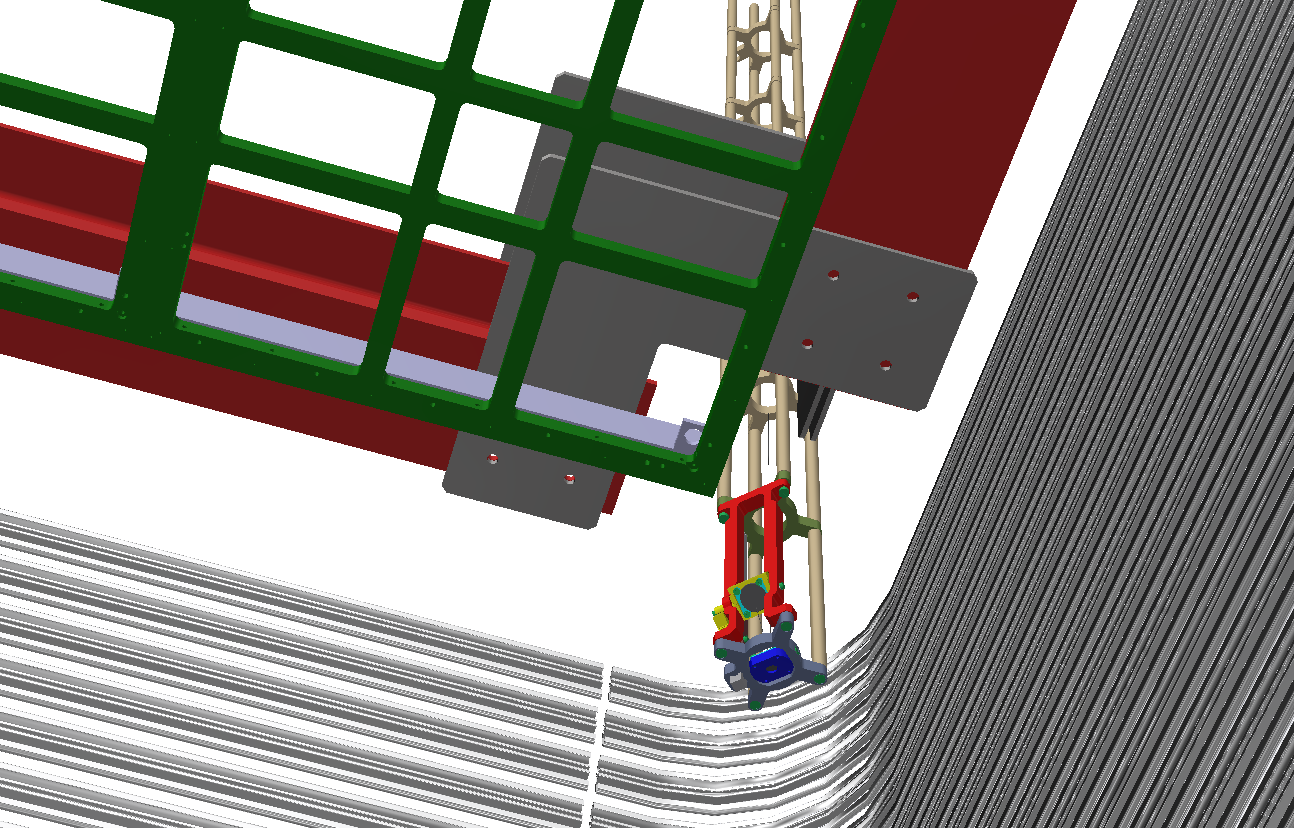
\includegraphics[width=0.49\linewidth]{LaserPositionCorner1.png}
\end{dunefigure}

\begin{dunefigure}[Laser calibration periscopes within the \dshort{dp} \dshort{tpc} side]{fig:LaserPositionSide}
{CAD illustration of the calibration periscopes within the \dword{dune} \dword{dp} \dword{tpc} side. 
%Left: Location on the corner. Right: Location on the side. 
Left: View from top. Right: View from bottom.}
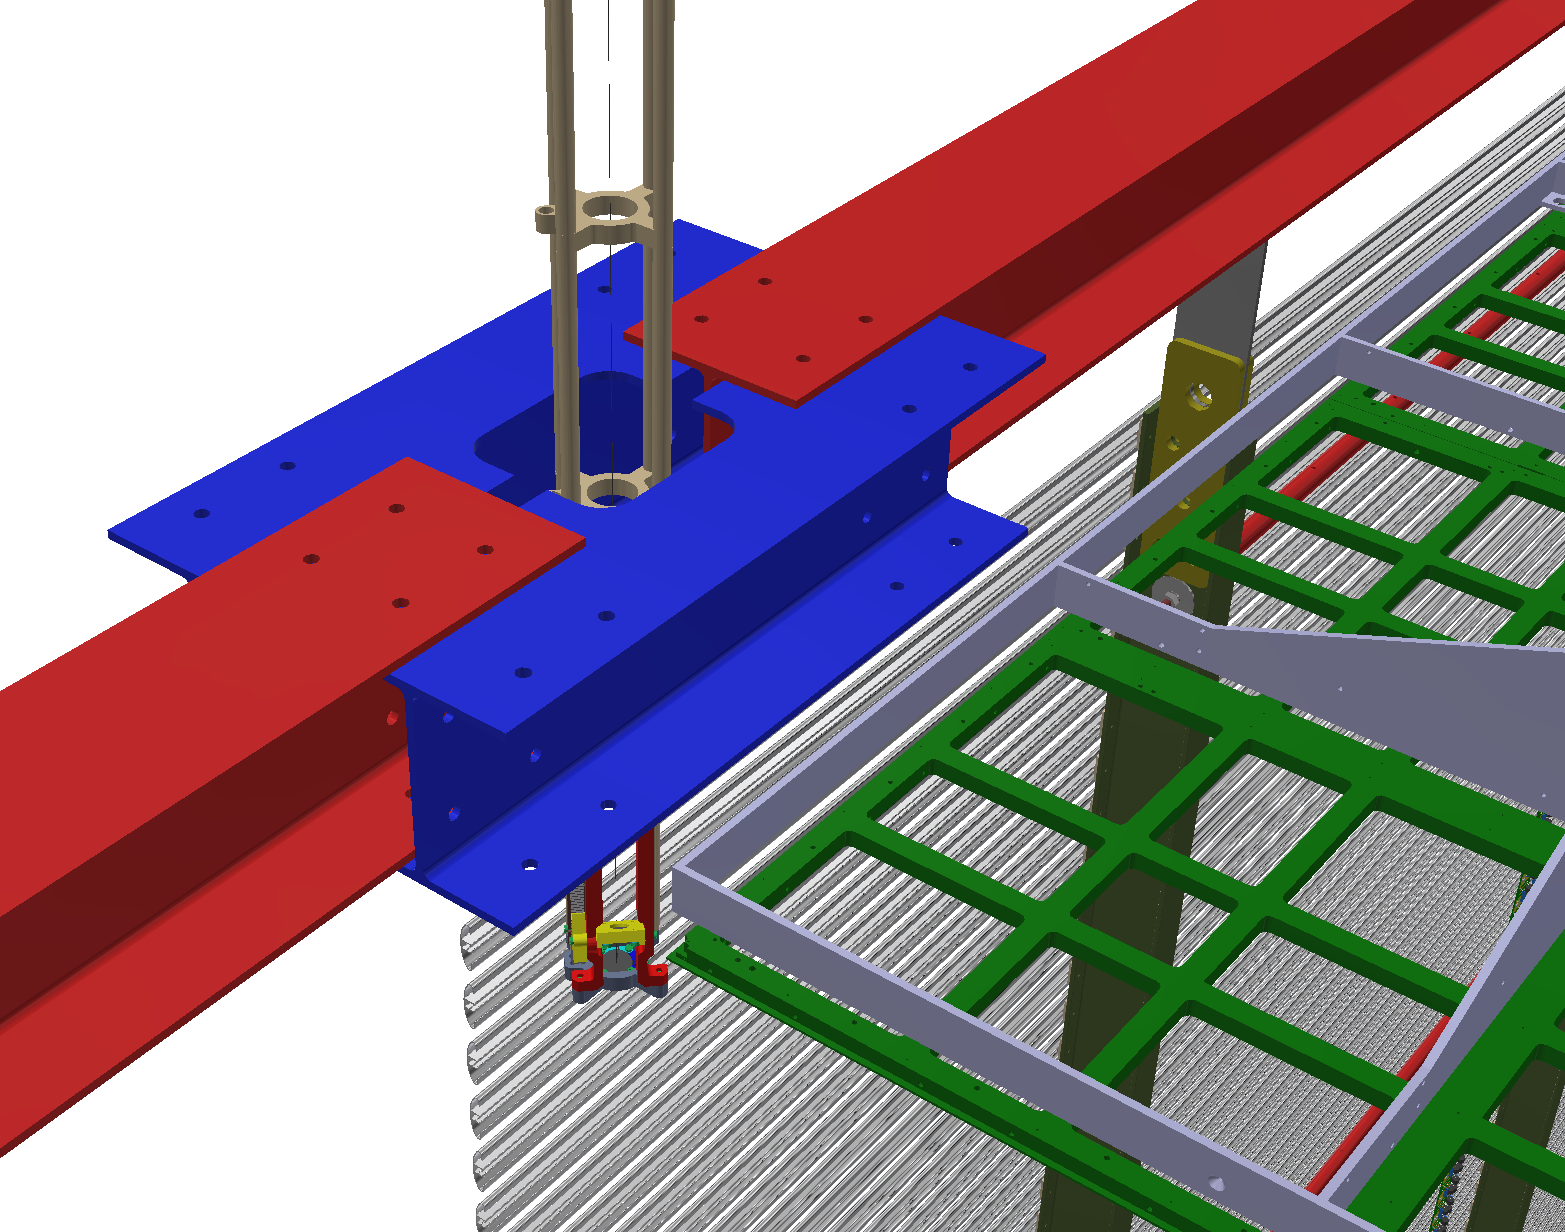
\includegraphics[width=0.49\linewidth]{LaserPositionSide.png}
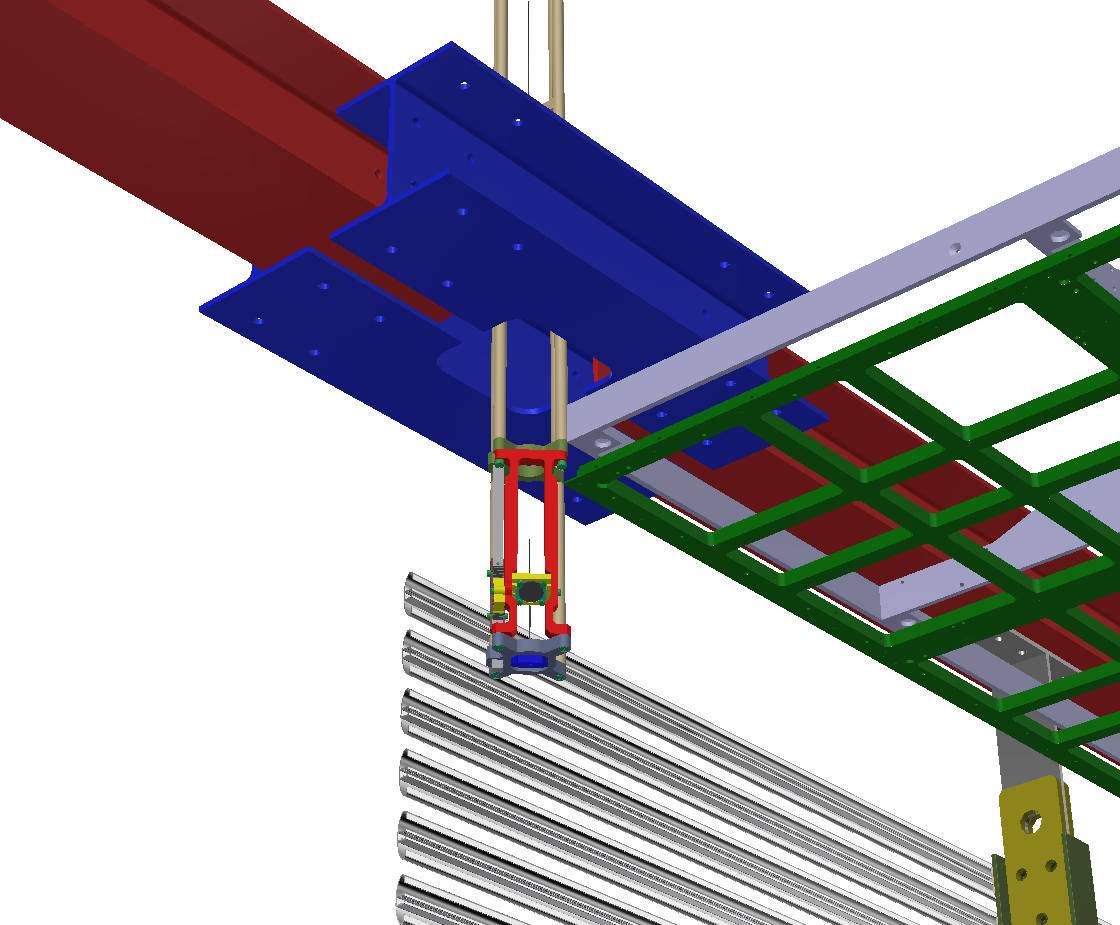
\includegraphics[width=0.49\linewidth]{LaserPositionSide1.png}
\end{dunefigure}


The goal of the mechanical design of the system is to achieve a precision close to that of the \dword{tpc} position measurements, so that no single factor dominates %in 
the overall systematics. The starting point of the laser beams is given by the position of the mirror in the periscope, which is known from construction drawings, warm surveys and cool down calculations. The angle of the beam is given by the angles ($\theta$, $\phi$) of the mirror, which are set by the periscope motors and read out by the encoders. 
For \dword{microboone}, reference~\cite{bib:chen2018} quotes a very good \SI{0.05}{\mrad} precision (\SI{0.5}{\milli\m} at \SI{10}{\m}) from the encoders alone, and an overall pointing precision of \SI{2}{\milli\m} at \SI{10}{\m}, driven mostly by beam size and divergence. In fact, with a \SI{0.5}{\mrad} divergence, we expect the beam to be \SI{5}{\milli\m} wide at \SI{10}{\m}.
In \dword{dune}, we aim to reach a similar precision. This will require a number of design and installation considerations: having encoders of similar high accuracy, carrying out surveys in various reference frames, and a capability to do location checks with a precision of about \SI{5}{\milli\m}  at \SI{20}{\m} from the beam origin. Therefore we aim to have a system that can locate the beam end point in few positions and attached to different references, at least one per drift volume and laser beam. The independent laser beam location system is described in Section~\ref{sec:dp-calib-sys-las-loc}. 

A scan of the full detector using \num{10}$\times$\num{10}$\times$\SI{10}{\cubic\cm} volume elements requires a number of tracks on the order of \num{4e5} and can take about two days. Shorter runs could be done to investigate specific regions. Sampling granularity, and therefore the amount of data taken, depends on \dword{daq} requirements. In fact, to even be able to record the desired \num{4e5} tracks, a dedicated data reduction algorithm must be devised, so that only a drift window of approximately \SI{100}{\micro\s}
of data is recorded; the position of that window depends on beam position as well as the direction and \dword{crp} sections being read out. More details on this are given in Section~\ref{sec:dp-calib-daqreq}.



%%%%%%%%%%%%%%%
\subsubsection{Measurement Program}
\label{sec:dp-calib-sys-las-ion-meas}

This section describes the methods used to measure 
%drift velocity and \efield 
parameter maps and their expected precision, given the design outlined above.

\paragraph{\efield and drift velocity measurement}
The method for \efield measurement is based on the measurement of apparent position displacements of the straight laser tracks. The laser produces straight tracks with a known starting position and direction. If, when reconstructed under the assumption of uniform and homogeneous drift velocity, any deviations from that are observed, they are attributed to \efield distortions. 

The first step in the analysis~\cite{bib:uBlaser2019} is to obtain a field of position displacements by comparing the known and reconstructed tracks. If two crossing tracks are used, the displacement vector is simply given by the vector connecting the point where the reconstructed tracks cross and the point where the known tracks cross. However, since those displacements can vary both in direction and magnitude, there will be ambiguity in that determination if only one track is used in a given spatial region. An iterative procedure was developed by the \dword{microboone} collaboration~\cite{bib:chen2018,bib:uBlaser2019} to obtain a displacement map from a set of several non-crossing tracks from opposite directions. Following this, a set of drift velocity field lines, which are the same as \efield lines, can be obtained from the displacement map, assuming that all charge deposits along a field line will be collected in the same position. Using the relationship between \efield and drift velocity~\cite{Li:2015rqa,Walkowiak:2000wf}, we can then also obtain the magnitude of the \efield.

Since the observed position distortion in one location depends on \efield distortions in many locations along the drift path, this method of analysis clearly requires the acquisition of data from many different tracks crossing each detector drift volume at many different angles. 

Therefore, the precision with which the \efield distortions can be measured depends on the precision with which we can know the laser track position and the \dword{tpc} position reconstruction precision.
The \dword{tpc} precision in the $y$, $z$ coordinates is given primarily by the \dword{crp} strip spacing of \dpstrippitch and lateral diffusion, which can be up to \SI{4.4}{\milli\m} for the maximum drift of \dpmaxdrift and nominal \efield of \dpnominaldriftfield.
It is slightly better than that (approximately \SI{2}{\milli\m}) on the $x$ (drift) coordinate, determined by the \fepeaktime peaking time of the front-end electronics.
Given infinite laser positioning accuracy, the smallest measurable \efield distortions would be those that cause displacements of approximately \SI{2}{\milli\m} in $x$ and \SI{5}{\milli\m} in $y$, $z$. The precision for the drift velocity distortions depends on the size of the spatial region where they are present. For distortions present in regions of \SI{0.5}{\m} and larger, drift velocity distortions can therefore be measured with an accuracy of \SI{1}{\%} in $y$, $z$ and \num{0.4}\% in $x$. In $y$, $z$, \SI{1}{\%} precision on drift velocity distortions translates to \SI{1}{\%} precision on the transverse field distortions. Along $x$, one must consider that, at \dpnominaldriftfield, a \SI{1}{\%} change in \efield leads to a \SI{0.375}{\%} change in drift velocity. Therefore, finally, this means that the smallest measurable distortions given the \dword{tpc} design (\dword{crp} pitch, timing precision) are \SI{1}{\%} in \efield if they are present in regions of \SI{0.5}{\m} and larger. Smaller field distortions could in principle be measurable if they are present over larger regions because their effect accumulates over the drift path.
On one hand, this gives us an ultimate limit to the \efield precision achievable with the laser system, but on the other hand, because these \dword{tpc} precision considerations apply to physics events also, this tells us an \efield precision much more than \SI{1}{\%} should not have an effect on physics.

\paragraph{Charge-based measurements}

Electron drift-lifetime~\cite{bib:uBlifetime, Antonello:2014eha} is the parameter that governs the dependence of the amount of collected charge on the drift time. A possible measurement of electron drift-lifetime would therefore require a very good control over the charge profile of the ionization laser tracks. This was achieved in a small scale experiment that measured lifetime with laser beams~\cite{Ereditato:2013xaa}, but is harder with longer distances. The charge produced by the laser tracks along its path depends on distance because the light intensity is reduced due to beam divergence and scattering, as well as non-linear effects such as the self-focusing, or Kerr effect. For this reason, the first steps in any laser-based charge measurement are a fine-tuning of the laser intensity in order to reduce self-focusing to a minimum, and ``charge profile calibration scan'' which consists of acquiring tracks parallel to the \dword{crp}. In order to get good statistical precision, several tracks could be acquired, in the same or different direction, but always parallel to the \dword{crp} in order to factorize out any effect from electron drift-lifetime. This set of data provides a calibrated laser beam charge profile that can then be used to analyse and normalize the measured charge profile from tracks that do have an angle with respect to the \dword{crp} and therefore span different drift times.

As for electron-ion recombination, since the $dE/dx$ for laser beams is much smaller than for charged particles, the effect should also be much smaller. However, that small effect has been observed~\cite{Badhrees:2010zz}, so a similar method than described above could be used to evaluate any dependence of the electron-ion recombination factor on the angle $\phi$ between the track and the electric field, that is predicted in some models~\cite{Acciarri:2013met}. This would entail taking data with tracks as parallel as possible to the \efield, in order to enhance the angular dependence term on the recombination expression (that goes with $1/sin \phi$), and to compensate for the smaller $dE/dx$ for laser beams.






